\chapter{Niet-Programmeerbare Processoren}
\chapterquote{We accepteren nu het feit dat leren een levenslang proces is om op de hoogte te blijven van veranderingen. En de meest urgente taak is mensen te leren hoe te leren.}{Peter F. Drucker, Amerikaans management consultant en auteur (1909-)}
\begin{chapterintro}
In de twee vorige hoofdstukken hebben we componenten gebouwd met een beperkte functionaliteit. De combinatorische schakelingen laten ons toe om schakelingen te ontwerpen die een rekenkundige operatie uitvoeren, maar we hebben geen geheugen beschikbaar om tussenresultaten in op te slaan. Het hoofdstuk over sequenti\"ele schakelingen maakt het mogelijk om schakelingen te ontwerpen met een geheugen. De meeste problemen hebben echter zeer grote toestandsruimtes (een 32-bit getal heeft meer dan vier miljard toestanden). Daarom volstaan de methodes uit dit hoofdstuk niet om een component te ontwikkelen die iets functioneel doet. Daarvoor zullen we methodes op een hoger niveau introduceren, dat van een niet-programmeerbare processor. Een niet programmeerbare processor voert een algoritme uit die op voorhand gekend is. Hierdoor kunnen we optimaal gebruik maken van de hardware en zoveel mogelijk instructies tegelijk uitvoeren. Het nadeel is dat eenmaal de processor geproduceerd is, we geen andere problemen met het component kunnen uitvoeren.
\end{chapterintro}
\minitoc[n]
\section{De Niet-Programmeerbare Processor}
Alvorens we de bouw van zo'n processor verder uitwerken, dienen we eerst enkele concepten te formaliseren. Allereerst ontleden we in deze sectie uit welke delen zo'n processor is opgebouwd. Vervolgens zullen we in sectie \ref{s:descriptionFSMD} een methode ontwikkelen om een algoritme formeel weer te geven. Deze beschrijving zal toelaten het algoritme later om te zetten naar een processor. In sectie \ref{s:memoryFSMD} ten slotte zullen we extra geheugencomponenten introduceren die we nodig zullen hebben bij de bouw van een processor.
\subsection{Algemene Structuur}
Een \termen{Niet-programmeerbare processor}, ofwel \termen{Finite State Machine with Data path (FSMD)} bestaat grofweg uit twee delen:
\begin{itemize}
 \item Een \termen{datapad}: een component die bewerkingen (rekenkundig, aritmetisch,...) uitvoert en de resultaten opslaat in tijdelijk geheugen.
 \item Een \termen{controller}: een component die het datapad aanstuurt. Het zegt welke actie op welk moment moet ondernomen worden.
\end{itemize}
In dit hoofdstuk is de controller niet programmeerbaar. Dat wil zeggen dat de controller telkens hetzelfde programma uitvoert. Dit betekent echter niet dat er een vaste cyclus in de controller zit. De controller kan afhankelijk van de waarden die in de geheugens van het datapad zitten, of van ingangen van de processor beslissen om andere acties te ondernemen. Een controller is dus een sequenti\"ele schakeling ofwel finite state machine. De synthese van een finite state machine werd in het hoofdstuk \ref{ch:SeqComp} reeds besproken. Uiteraard zullen we de karakteristieken die eigen zijn aan controllers in dit hoofdstuk bespreken.
\paragraph{}
Het spreekt voor zich dat de controller en het datapad continu data met elkaar uitwisselen. Enerzijds geeft de controller instructies aan het datapad. De groep signalen waarmee een controller een datapad aanstuurt noemen we het ``\termen{instructiewoord}'' ofwel ``\termen{controle-signalen}''. Anderzijds zullen de instructies vaak afhangen van de toestand van variabelen opgeslagen in het datapad. De verzameling van signalen die het datapad over zijn variabelen doorstuurt naar de controller noemen we ``\termen{statussignalen}''.
\paragraph{}
Een processor voert operaties uit op data. Deze data moet op de een of andere manier ingelezen worden in de processor. De verzameling ingangen waarmee we data vanuit de omgeving in het datapad injecteren noemen we de ``\termen{data-ingangen}''. Verder zullen we vaak ook informatie aan de controller moeten meedelen: we denken bijvoorbeeld aan een signaal die actief wordt wanneer alle data ingelezen is, en het algoritme kan uitgevoerd worden. Deze signalen noemen we ``\termen{controle-ingangen}''. Daarnaast willen we ook de resultaten kunnen uitlezen. Hiervoor voorzien we een reeks signalen vanuit het datapad, deze signalen noemen we ``\termen{data-uitgangen}''. Tot slot zijn we soms ook ge\"interesseerd in de toestand van het algoritme. We zullen bijvoorbeeld enkel data uitlezen indien het algoritme afgelopen is. De controller kan informatie over het algoritme naar buiten brengen via ``\termen{controle-uitgangen}''. De verschillende informatiestromen tussen het datapad en de controller en de processor en zijn omgeving beschrijven we op figuur \ref{fig:processorInformationStreams}.
\begin{figure}[hbt]
\centering
\subfigure[Processor]{
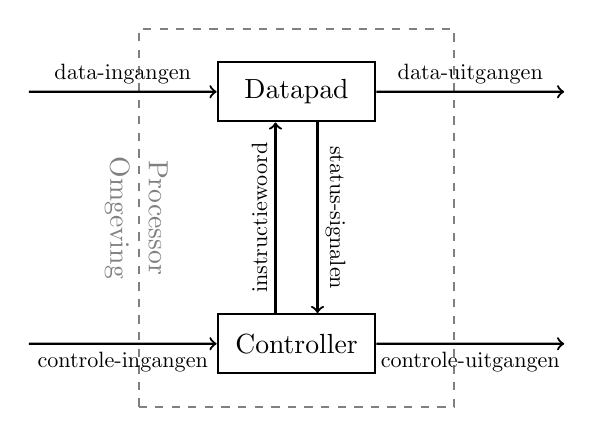
\begin{tikzpicture}[scale=0.8]
\draw[gray,dashed,thick] (-2.5,-3) rectangle (2.5,3);
\draw (-2.5,0) node[rotate=-90,gray,anchor=south]{Processor};
\draw (-2.5,0) node[rotate=-90,gray,anchor=north]{Omgeving};
\node[rectangle,thick,draw=black,minimum width=2 cm,minimum height=0.75 cm] (D) at (0,2) {Datapad};
\node[rectangle,thick,draw=black,minimum width=2 cm,minimum height=0.75 cm] (C) at (0,-2) {Controller};
\draw[->,thick] (D.south -| 0.3333,0) to node[midway,sloped,above,scale=0.8]{status-signalen} (C.north -| 0.3333,0);
\draw[->,thick] (C.north -| -0.3333,0) to node[midway,sloped,above,scale=0.8]{instructiewoord} (D.south -| -0.3333,0);
\draw[<-,thick] (C.west) to node[below,midway,scale=0.8]{controle-ingangen} (-4.25,-2);
\draw[->,thick] (C.east) to node[below,midway,scale=0.8]{controle-uitgangen} (4.25,-2);
\draw[<-,thick] (D.west) to node[above,midway,scale=0.8]{data-ingangen} (-4.25,2);
\draw[->,thick] (D.east) to node[above,midway,scale=0.8]{data-uitgangen} (4.25,2);
\end{tikzpicture}
\label{fig:processorInformationStreams}}
\subfigure[Datapad]{
\begin{tikzpicture}[scale=0.8]
\draw[gray,dashed,thick] (-3.5,-3) rectangle (3.5,3);
\draw (-3.5,1.3) node[rotate=-90,gray,anchor=south]{Datapad};
\draw (-3.5,1.3) node[rotate=-90,gray,anchor=north]{Omgeving};
\node[rectangle,thick,draw=black,minimum width=2 cm] (T) at (0,1.25) {Tijdelijk geheugen};
\node[trapezium,thick,draw=black] (O) at (0,0) {Operatorverbindingen};
\node[rectangle,thick,draw=black,minimum width=2 cm] (F) at (0,-1.25) {Functionele eenheden};
\node[minimum width=2 cm] (RA) at (0,-2.5) {Resultaatverbindingen};
\node[minimum width=2 cm,white] (RB) at (0,2.5) {Resultaatverbindingen};
\draw[thick] (RA.north west) -- (O.bottom left corner |- RA.south) -- (RA.south east) -- ++(1,0) |- (RB.north west) -- (RB.south -| O.bottom left corner) -- (RB.south east) -- ++(0.5,0) |- (RA.north west);
\draw[thick,->] (RB) -- (T);
\draw[thick,->] (T) -- (O);
\draw[thick,->] (O) -- (F);
\draw[thick,->] (F) -- (RA);
\draw[<-,thick] (RA.west -| O.west) -- ++(-3,0);
\draw[<-,thick] (RB.west -| O.west) -- ++(-3,0);
\draw (-4,0) node[scale=0.8,anchor=south]{instructiewoord};
\draw (-4,-2.5) node[scale=0.8,anchor=south]{instructiewoord};
\draw (-4,2.5) node[scale=0.8,anchor=south]{externe-ingangen};
\draw (1.75,-3.5) node[scale=0.8,anchor=south]{externe-uitgangen};
\draw[<-,thick] (O.west) -- ++(-3,0);
\draw[->,thick] (RA) |- ++(3.5,-1);
% \draw[->,thick] (D.south -| 0.5,0) to node[midway,sloped,above]{status-signalen} (C.north -| 0.5,0);
% \draw[->,thick] (C.north -| -0.5,0) to node[midway,sloped,above]{instructiewoord} (D.south -| -0.5,0);
% \draw[<-,thick] (C.west) to node[below,midway]{controle-ingangen} (-4.5,-2);
% \draw[->,thick] (C.east) to node[below,midway]{controle-uitgangen} (4.5,-2);
% \draw[<-,thick] (D.west) to node[above,midway]{data-ingangen} (-4.5,2);
% \draw[->,thick] (D.east) to node[above,midway]{data-uitgangen} (4.5,2);
\end{tikzpicture}
\label{fig:datapadInformationStreams}}
\caption{Opbouw van een processor en datapad.}
\end{figure}
\paragraph{}
Door de controle-ingangen wordt de definitie van ``niet-programmeerbaar'' natuurlijk vaag. We zouden immers het toestandswoord van de controller in grote mate laten afhangen van de invoer die de controle-ingangen. Hierdoor kunnen we de processor toch programmeren. Het onderscheid is dan ook eerder een common-sense.
\subsection{Het Datapad}
Zoals we reeds hebben vermeld, kunnen we een controller modelleren als een eindige toestandsautomaat ofwel finite state machine. Een datapad daarentegen bestaat uit verschillende componenten:
\begin{itemize}
 \item \termen{Functionele Eenheden} ofwel \termen{Functional Units (FU)}: dit zijn schakelingen die berekeningen en aritmetisch operaties uitvoeren. Dit zijn dus de componenten die we in hoofdstuk \ref{ch:combinatoric} hebben besproken: optellers, ALU, schuifoperator,... Uiteraard kunnen we ook zelf functionele eenheden bouwen op de manier die we gezien hebben.
 \item \termen{Tijdelijke geheugens}: dit zijn componenten die de waarden waarop we bewerkingen uitvoeren voor enkele klokcycli kunnen vasthouden. Dit zijn bijvoorbeeld de registerbanken en RAM die we in sectie \ref{s:memoryFSMD} zullen invoeren. Het zijn groepen van flipflops die ons toelaten om op een hoger niveau te redeneren.
 \item \termen{Verbindingen}: de tijdelijke geheugens en de functionele eenheden wisselen informatie uit. Daarom hebben we twee types verbindingen nodig:
 \begin{itemize}
  \item \termen{Operandverbindingen}: dit zijn verbindingen die de waardes van de tijdelijke geheugens overbrengen als operanden van de functionele eenheden. De waarde van een register kan op die manier bijvoorbeeld gebruikt worden bij een optelling.
  \item \termen{Resultaatverbindingen}: het is de bedoeling dat de resultaten vervolgens in een tijdelijk geheugen opgeslagen worden. Resultaatverbindingen transporteren de resultaten van de functionele eenheden terug naar de tijdelijke geheugens. Sommige uitvoer kan ook weggeschreven worden naar de data-uitgangen. Ook de invoer van de data-ingangen wordt door deze verbindingen verwerkt.
 \end{itemize}
 Het spreekt voor zich dat de verbindingen beslissen welke geheugens als operanden en resultaatgeheugens dienen. Daarom zullen we ze implementeren als bussen met multiplexers en 3-state buffers. Deze bussen zullen dan worden aangestuurd door de controller.
\end{itemize}
Dit concept beschrijven we op figuur \ref{fig:datapadInformationStreams}.
\paragraph{}
In het datapad doen we dan ook niets anders dan waardes uit het tijdelijke geheugen inlezen, er een operatie van een functionele eenheid op uitvoeren en vervolgens in een tijdelijk geheugen plaatsen. Dit proces noemen we ook wel de ``\termen{registertransfer}'' en formaliseren we als:
\begin{equation}
\mbox{register}_a\leftarrow\mbox{FU}_a\left(\mbox{register}_{a_1},\mbox{register}_{a_1},\mbox{register}_{a_2},\ldots,\mbox{register}_{a_n}\right)
\end{equation}
In het eerste hoofdstuk hebben we reeds vermeld dat we schakelingen bij het bouwen van een processor beschrijven op registertransfer-niveau. Dit betekent dat we bijvoorbeeld abstractie zullen maken van flipflops en zullen werken met registers. Ook zullen we details als het aantal bits die een opteller nodig heeft verwaarlozen. Deze nieuwe notatiestijl zullen we geleidelijk invoeren.
\section{Formeel Beschrijven van een Algoritme}
\label{s:descriptionFSMD}
Alvorens we een processor kunnen bouwen die een algoritme uitvoert, moeten we eerst een formeel algoritme kunnen opstellen. Dit algoritme vertrekt altijd vanuit een probleemstelling. Hoe we een probleemstelling omzetten naar een algoritme behoort niet tot de inhoud van deze cursus\footnote{Het omzetten van een probleem in een algoritme is geen exacte wetenschap. Het is een vaardigheid die wel geoefend kan worden. Hiervoor bestaan er andere cursussen.}.
\subsection{Leidend Voorbeeld: Deler}
Als leidend voorbeeld doorheen dit hoofdstuk zullen we een processor bouwen die natuurlijke getallen kan delen. Uiteraard zouden we hiervoor een combinatorische schakeling kunnen bouwen. We zullen echter een algoritme beschouwen om de berekening te maken. De processor heeft 2 32-bit ingangen die het deeltal en de deler inlezen. Verder bevat het ook een controle-ingang. Zolang we een laag signaal op de controle-ingang aanleggen betekent dit dat er geen correcte invoer op de data-ingangen staat. Pas wanneer we een hoog signaal aanleggen zal het algoritme dus een deling uitvoeren. Verder bevat de processor ook 2 32-bit uitgang om het quoti\"ent en de rest naar buiten te brengen, en een controle uitgang die hoog wordt op het moment dat het algoritme het quoti\"ent en de rest heeft berekend. Zolang de controle-uitgang dus laag is, is het algoritme nog bezig met de berekening. We maken de assumptie dat de deler nooit gelijk is aan 0. Het algoritme die dan vervolgens het deeltal en de deler omzet in het quoti\"ent en rest staat op \algoref{alg:devisionFSMD}.
\begin{algorithm}[hbt]
\caption{Delen van twee $n$-bit getallen.}\label{alg:devisionFSMD}
\begin{algorithmic}[1]
\Function{Division}{$N,D$}
\State $Q\gets 0$
\State $R\gets 0$
\For{$i\gets n-1...0$}
\State $R\gets 2\times R$
\State $R\left[0\right]\gets N\left[i\right]$
\If{$R\geq D$}
\State $R\gets R-D$
\State $Q\left[i\right]\gets 1$
\EndIf
\EndFor
\State \Return $\left(Q,R\right)$
\EndFunction
\end{algorithmic}
\end{algorithm}
We gaan niet in op de precieze werking van het algoritme. Indien we een index opvragen of zetten bij een variabele zoals $V\left[i\right]$ betekent dit dat we een operatie op de $i$-de bit uitvoeren. Dit algoritme is echter niet geschikt voor een processor. Een processor voert immers continu het programma uit. Bovendien wordt hier niet gewacht tot er invoer op de data-ingangen staat. Daarom zullen we het algoritme herschrijven. We beschouwen hierbij de controle-ingang $ci$ en de controle-uitgang $co$.
\subsection{Toestandsbeschrijving}
\subsection{Toestand-Actie Tabel}
\subsection{ASM-Schema}
\section{Geheugencomponenten}
\label{s:memoryFSMD}
\subsection{Registerbank}
\subsection{Random Access Memory (RAM)}
\subsection{Stack (Last-In-First-Out)}
\subsection{Queue (First-In-First-Out)}
\section{Synthese van een Niet-Programmeerbare Processor}
\label{s:syntheseFSMD}
\section{Tijdsgedrag}
\label{s:timeFSMD}